\documentclass[12pt]{article}
\expandafter\def\csname
ver@l3backend.sty\endcsname{}

\usepackage{geometry}

\usepackage{tikz}
\usepackage{amsmath}
\usepackage{amsthm}
\usepackage{amssymb}
\usepackage{mathtools}
\usepackage{setspace}
\usepackage{graphicx}
\usepackage{subcaption}
\usepackage{epigraph}
\usepackage{etoolbox}
\usepackage{apacite}
\usepackage{xcolor}
\usepackage{graphicx}
\usepackage{subcaption}
\usepackage[utf8]{inputenc}
\usepackage{fontspec}
\usepackage{l3backend}
\usepackage{polyglossia}
\usepackage{testhyphens}
\setmainlanguage{finnish}
\addto\captionsfinnish{\renewcommand{\figurename}{Kuvio}}

\newcommand{\lastdatamonth}{\input{parameters/lastdatamonth.txt}} 
\newcommand{\firstdatamonth}{\input{parameters/firstdatamonth.txt}} 

\newcommand{\lastdataquarter}{\input{parameters/lastdataquarter.txt}} 
\newcommand{\firstdataquarter}{\input{parameters/firstdataquarter.txt}} 


 \geometry{
 a4paper,
 % total={165mm,230mm},
 left=25mm,
 top=25mm,
 right=25mm
 }
 
\title{Alueellisesta ja ammatillisesta kohtaannosta}
\date{January 2022}
\author{Juho Alasalmi \\ 
Pellervon Taloustutkimus\\
\textcolor{red}{Luonnos, kommentit tervetulleita.}}



\begin{document}

\maketitle

\begin{abstract}
Arvioin työmarkkinoiden alueellisen ja ammatillisen kohtaannon kehitystä Suomessa vuodesta 2006 alkaen. Muodostan kohtaanto-ongelman suuruutta mittaavan indeksin \cite{csahin2014mismatch}, joka kuvaa kuinka epätasapainoisesti työttömät työnhakijat ja avoimet työpaikat ovat sijoittuneet eri alueille ja eri ammatteihin verrattuna tilanteeseen, jossa alueellinen tai ammatillinen liikkuvuus eivät olisi rajoitteita. Arvioin sekä alueellisen että ammatillisen kohtaanto-ongelman trendinomaisesti pienentyneen 2000-luvun aikana. Kokonaisuudessaa työmarkkinoiden kohtaanto on Beveridge-käyrällä mitattuna kuitenkin heikentynyt. Kohtaannon heikentyminen ei siten tuskin johdu työmarkkinoiden välisen liikkuvuuden vähentymisestä vaan työmarkkinoiden sisäisen kohtaannon heikentymisestä. 
\end{abstract}


\setstretch{1.2}

\section{Johdanto} \label{section:johdanto}

Työmarkkinoiden kohtaannon parantaminen on usein mainittu yhtenä keskeisimpänä työllisyysasteen nostoon tähtäävistä keinoista. Mutta kuinka suuri kohtaanto-ongelma oikeastaan on? Kuinka se on muuttunut ajassa? Kumpi on merkittävämpi: ammatillinen vai alueellinen kohtaanto-ongelma? \citeA{csahin2014mismatch} ovat kehittäneet indeksin, jolla kohtaanto-ongelmien suuruutta voidaan arvioida. Tässä heidän indeksinsä yksinkertaisimmillaan ja sovellettuna Suomen työmarkkinoille.

Työttömien työnhakijoiden ja avoimien työpaikkojen kohtaamattomuus työmarkkinoilla voidaan ensinnäkin jakaa työmarkkinoiden välisiin kohtaanto-ongelmiin ja työmarkkinoiden sisäisiin kohtaanto-ongelmiin. Työmarkkinoiden väliset kohtaanto-ongelmat syntyvät, kun työnhakijat eivät liiku työmarkkinoiden välillä silloin, kun liikkuvuus työmarkkinoiden välillä edistäisi heidän työllistymistään. Tällainen tilanne syntyy, kun joillain työmarkkinoilla on pulaa työvoimasta, kun taas joillain työmarkkinoilla työttömiä suhteessa avoimiin työpaikkoihin on paljon. Työmarkkinoiden väliset kohtaanto-ongelmat ovat erityisesti alueellisia tai ammatillisia, riippuen siitä ajatellaanko työmarkkinoiden muodostuvat alueellisesti vai ammatillisesti.

Työmarkkinoiden sisäiset kohtaanto-ongelmat puolestaan syntyvät, kun avoin työpaikka ja työnhakija eivät kohtaa siten että työnhakija työllistyisi tähän avoimeen työpaikkaan, vaikka kohtaaminen ei edellyttäisi työmarkkinoiden välistä liikkuvuutta. Tällaiset työmarkkinoiden sisäiset kohtaanto-ongelmat voivat syntyä esimerkiksi etsintäkitkojen tai työllistymisen kannattamattomuuden vuoksi. 
Tämä teksti keskittyy työmarkkinoiden välisten kohtaanto-ongelmien mittaamiseen. Työmarkkinoiden sisäisiä kohtaanto-ongelmia ovat arvioineet \citeA{pehkonen2018kohtaanto}. Siten kohtaanto-ongelmalla tarkoitetaan tässä tekstissä pääasiassa työmarkkinoiden välistä, alueellista tai ammatillista, kohtaanto-ongelmaa.

\subsection{Kohtaanto-ongelman mittaaminen} \label{section:kohtaanto-ongelman mittaaminen}

Aloitetaan ongelmaa yksinkertaistavalla ajatusleikillä. Ajatellaan, että Suomessa on $N$ kappaletta työmarkkinoita. Tarkastellaan siis ainoastaan mahdollisia Suomen sisäisiä työmarkkinoiden kohtaanto-ongelmia. Nämä työmarkkinat voivat määrittyä alueen, ammatin tai alueen ja ammatin perusteella. Esimerkiksi ekonomistit ja työpaikat ekonomisteille voidaan ajatella olevan yksi työmarkkina. Työmarkkinoista voidaan tehdä myös pienempiä ajattelemalla Helsingissä asuvien ekonomistien ja Helsingissä olevien ekonomistitöiden muodostavan yhden työmarkkinan. Oletus on, että avoimet työpaikat voidaan täyttää vain saman työmarkkinan työttömillä ja työttömät voivat hakevat töitä ainoastaan oman työmarkkinansa sisältä. Vain samalla työmarkkinalla olevat työttömät ja avoimet työpaikat voivat kohdata ja liikkuvuutta työmarkkinoiden välillä ei siis ole. Huomaa, että sitä rajoittavampi oletus työmarkkinoiden välisestä liikkumattomuudesta on, mitä pienemmäksi työmarkkinat määritellään. Yksinkertaisuuden vuoksi ajatellaan myös, että kaikki työttömät ja avoimet työpaikat työmarkkinalla ovat samanlaisia siten, että työmarkkinan työttömillä on kaikilla sama todennäköisyys työllistyä ja työmarkkinan avoimilla työpaikoilla on kaikilla sama todennäköisyys täyttyä.

Otetaan yksi työmarkkina ja nimetään se $n$:ksi. Ajanhetkellä $t$ tällä työmarkkinalla on $v_{nt}$ avointa työpaikkaa ja $u_{nt}$ työtöntä työnhakijaa. Koska työttömien työnhakijoiden työpaikkojen etsintä ja työnantajien työntekijöiden etsintä vaatii aikaa, avoimet työpaikat eivät täyty välittömästi. Kuvataan tätä työmarkkinoiden sisäistä kitkaa yksinkertaisesti kohtaantofunktiolla ja sanotaan, että avoimet työpaikat ja työttömät työnhakijat löytävät toisensa vauhtia, joka riippuu työttömien työnhakijoiden ja avoimien työpaikkojen määrästä: 
\begin{align*}
h_{nt} = v_{nt}^\alpha v_{nt}^{1-\alpha}
\end{align*}
eli toisin sanoen työtön työnhakija työmarkkinalla n aikavälillä t ja t+1 työllistyy todennäköisyydellä 
\begin{align*}
\frac{h_{nt}}{u_{nt}} = \left ( \frac{v_{nt}}{u_{nt}} \right ) ^\alpha,
\end{align*}
missä $h_{nt}$ on ajanhetkien $t$ ja $t+1$ välillä työllistyneiden (ja täyttyneiden työpaikkojen) määrä ja $a$ on parametri, joka määrää kuinka työllistymisen todennäköisyys riippuu työmarkkinan kireydestä. Työllistymisen todennäköisyys työmarkkinalla laskee työttömien määrän kasvaessa tai avoimien työpaikkojen määrän laskiessa. Useat tutkimukset ovat estimoineet parametrin a arvoa. \citeA{csahin2014mismatch} käyttävät näihin tutkimuksiin perustuen arvoa 0,5, joten asetetaan $a = 0,5$. Alla tulosten herkkyyttä tämän parametrin arvolle testataan ja käy ilmi, että tämä parametrin arvo 0,5 asettaa ylärajan kohtaanto-ongelman suuruudelle.

Ajatuksena kohtaanto-ongelman suuruuden kartoittamisessa on verrata työttömien työnhakijoiden todellista jakautumista työmarkkinoille $N$ sellaiseen jakautumiseen, jossa kohtaanto-ongelmaa ei olisi. Kohtaanto-ongelmaa ei ole, jos työmarkkinalta toiselle liikkuminen ei lisää työllisyyttä. Kuvitellaan siten, että voimme uudelleensijoittaa työttömät työnhakijat työmarkkinoille siten, että kohtaanto-ongelma poistuisi. Merkitään työmarkkinalla n ajanhetkellä t olevien työttömien määrää tässä ideaalitilanteessa $u_{nt}^*$.

Ideaalitilanteessa työllistymisen todennäköisyys jokaisella työmarkkinalla olisi sama. Jos näin ei olisi, silloin jollakin työmarkkinalla työllistymisen todennäköisyys olisi suurempi kuin jollakin toisella ja kohtaantoa voisi parantaa siirtämällä työttömiä edelliseltä työmarkkinalta jälkimmäiselle. Siten työttömien ideaalijako työmarkkinoille ajanhetkellä $t$ täyttää ehdon:
\begin{align}
\frac{v_{nt}}{u_{nt}^*} = \frac{v_{mt}}{u_{mt}^*} \textrm{ kaikilla työmarkkinoilla } n, m \in N
\label{eq:dfwewe}
\end{align}
Työllistymisen todennäköisyys jokaisella työmarkkinalla tulisi siis olla sama ja tämän todennäköisyyden täytyy siten olla sama kuin työllistymisen todennäköisyys koko maassa:
\begin{align*}
\frac{h_{nt}^*}{u_{nt}^*} = \left ( \frac{v_{nt}}{u_{nt}^*} \right )^{0.5} = \left ( \frac{v_{t}}{u_{t}^*} \right )^{0.5} \textrm{ kaikilla } n \in N
\end{align*}
missä $\sum_{n\in N} v_{nt}=v_t$ ja $\sum_{n\in N} u_{nt}^*=u_t^*$. Ajanhetkien $t$ ja $t+1$ välillä koko maassa työllistyy kohtaanto-ongelman vallitessa
\begin{align}
h_t=\sum_{n\in N} h_{nt}=\sum_{n\in N}\left(v_{nt}u_{nt}\right)^{0.5}
\end{align}
työtöntä työnhakijaa, mutta jos ehdon (\ref{eq:dfwewe}) mukaisesti kaikki $u_t$ työtöntä uudelleenjaetaan työmarkkinoille, tänä aikana työllistyy
\begin{align}
h_t^*=\sum_{n\in N} h_{nt}^*=\sum_{n\in N}\left(v_{nt}u_{nt}^*\right)^{0.5}=\left(v_tu_t\right)^{0.5}
\end{align}
työtöntä työnhakijaa. Huomaa, että ilman kohtaanto-ongelmaa työllistyneiden määrä on siis sama kuin, jos koko Suomessa olisi vain yksi työmarkkina. Kohtaanto-ongelman vuoksi $h_t^*-h_t$ työtöntä työnhakijaa ei siis työllisty ajanhetkien $t$ ja $t+1$ välillä. Määritellään kohtaanto-ongelman suuruutta mittaava indeksi kohtaanto-ongelman vuoksi työllistymättömien määrän suhteena työllistyvien määrään tilanteessa, jossa kohtaanto-ongelmaa ei olisi:
\begin{align}
M_t=\frac{h_t^*-h_t}{h_t^*}=1-\sum_{n\in N}\left(\frac{v_{nt}}{v_t}\frac{u_{nt}}{u_t}\right)^{0.5}.
\end{align}
Indeksi siis kertoo, kuinka suuri osa työllistymisistä jää tapahtumatta kohtaanto-ongelman vuoksi. Se kuvaa, kuinka epätasapainoisesti työttömät työnhakijat ja avoimet työpaikat ovat sijoittuneet eri alueille ja eri ammatteihin verrattuna tilanteeseen, jossa alueellinen tai ammatillinen liikkuvuus eivät olisi rajoitteita. 

Huomaa, että indeksin arvon muutokset ajassa johtuvat ainoastaan uusien avoimien työpaikkojen ja työttömien erilaisesta sijoittumisesta alueille ja ammatteihin ja ei siten riipu työmarkkinoiden sisäiseen tehokkuuteen vaikuttavista tekijöistä. Siten indeksi olettaa kohtaannon tehokkuuden säilyvän vakiona työmarkkinoiden sisällä. Eri ajankohdille laskettujen indeksien arvot siten vakioivat mahdolliset alueellisesta ja ammatillisesta kohtaannosta riippumattomat muutokset kohtaannon tehokkuudessa.

\subsection{Kohtaanto-ongelman suuruus Suomessa} \label{section:kohtaanto-ongelman suuruus suomessa}

Ensimmäinen käytännön kysymys indeksiä laskiessa aineistosta on työmarkkinoiden määrittely. Indeksi määrittelee kohtaanto-ongelman siten, että työntekijät ja avoimet työpaikat eivät liiku työmarkkinoiden välillä ollenkaan, mutta liikkuvat työmarkkinoiden sisällä ilman alueellisen tai ammatillisen liikkuvuuden rajoitteita. Tällaista työmarkkinajakoa ei luonnollisesti ole todellisuudessa olemassa, ja todellisuudessa työmarkkinoiden rajojen ylittämisessä on enemmänkin kyse liikkuvuuden vaikeudesta eikä niinkään sen mahdollisuudesta. Työmarkkinoita voitaisiin myös määritellä aineistolähtöisesti todellisen liikkuvuuden tai työnetsintäkäyttäytymisen perusteella kuten \citeA{marinescu2018mismatch} tekevät, mutta mielenkiintoista on myös määritellä eri kokoisia ja erilaisia työmarkkinoita ja nähdä, kuinka suureksi indeksi kullakin määritelmällä arvioi kohtaanto-ongelman. Kullekin työmarkkinamääritelmälle indeksi voi kuitenkin yliarvioida kohtaanto-ongelman suuruutta, koska se perustuu oletukseen, ettei työmarkkinoiden välillä ole liikkuvuutta, mutta toisaalta voi aliarvioida kohtaanto-ongelman suuruutta olettaessaan, ettei kohtaanto rajoita alueellista tai ammatillista liikkuvuutta työmarkkinan sisällä. 

Työ- ja elinkeinoministeriön Työnvälitystilasto tarjoaa Tilastokeskuksen välityksellä tietoa avoimien työpaikkojen ja työttömien työnhakijoiden sijainneista ja ammateista kuukausittain vuodesta 2006 eteenpäin \cite{svt2011}. Sekä avoimille työpaikoille että työttömille työnhakijoille on määritelty alue kunnan tarkkuudella sekä ammatti Kansallinen Ammattiluokitus 2010 -luokituksen 4-numerotason tarkkuudella. Laskelmat käyttävät näitä tietoja. Laskelmissa käytettävät koko maan tiedot ovat aina laskettu summaamalla ne alue- tai ammattikoodikohtaisista tiedoista, sillä indeksin laskennassa on tärkeää, että alue- tai ammattikohtaiset tiedot summautuvat koko maan tietoihin. Lisäksi avoimen aineiston suojatuille tiedoille on imputoitu arvoja. Tulokset eivät ole herkkiä näille imputoinneille.

\subsection{Alueellinen kohtaanto} \label{section:alueellinen_kohtaanto}

\begin{figure}
\centering
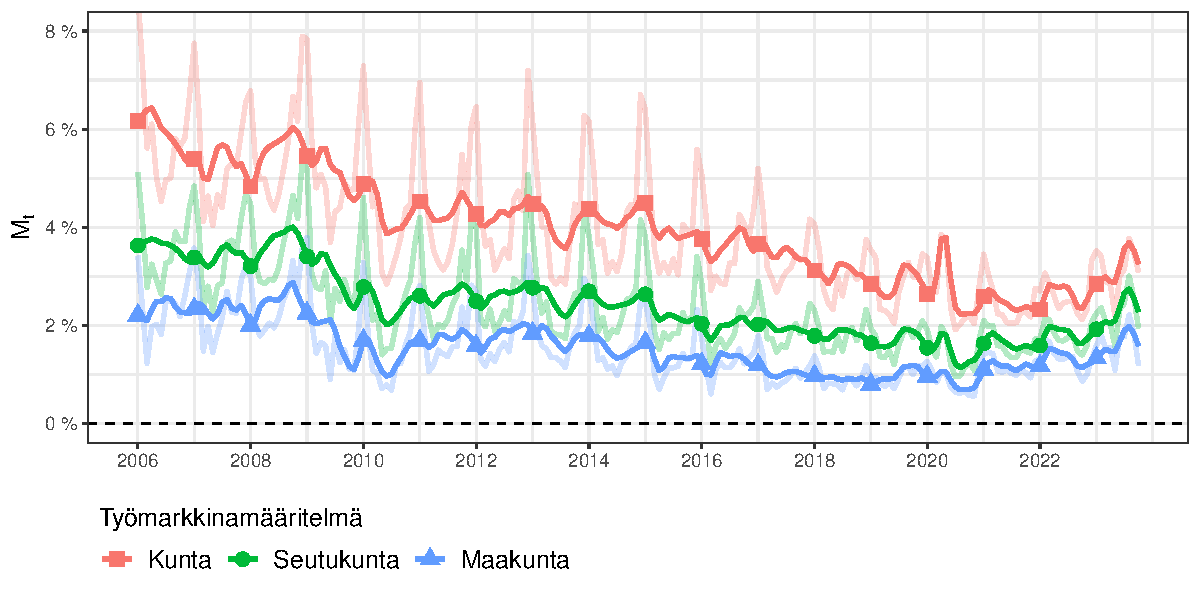
\includegraphics[scale = 0.8]{../kuviot/indeksi_alueittain.pdf}
    \caption{\textit{Kohtaanto-ongelman suuruutta mittaava indeksi ja sen trendi määrittelemällä työmarkkinoiden koostuvan kunnista, seutukunnista tai maakunnista.  \protect \firstdatamonth - \protect\lastdatamonth. Datalähde: Työnvälitystilasto, Tilastokeskus, taulukko 12r5 \protect \cite{svt2011}}}
   \label{fig:kdieksl}
\end{figure}

Tarkastellaan ensin alueellisen kohtaanto-ongelman laajuutta määrittelemällä työmarkkinoiden muodostuvan joko kunnista, seutukunnista tai maakunnista. Odotettavasti mitä laajemmaksi määrittelemme työmarkkinat, sitä pienemmäksi arvioimme alueellisen kohtaanto-ongelman, sillä työmarkkinan sisällä alueellista kohtaanto-ongelmaa ei oleteta olevan. Ääritapauksessa mikäli määrittelisimme koko Suomeen vain yhden työmarkkinan, niin arvioisimme alueellisen kohtaanto-ongelman suuruuden nollaksi.

\begin{figure}
\centering
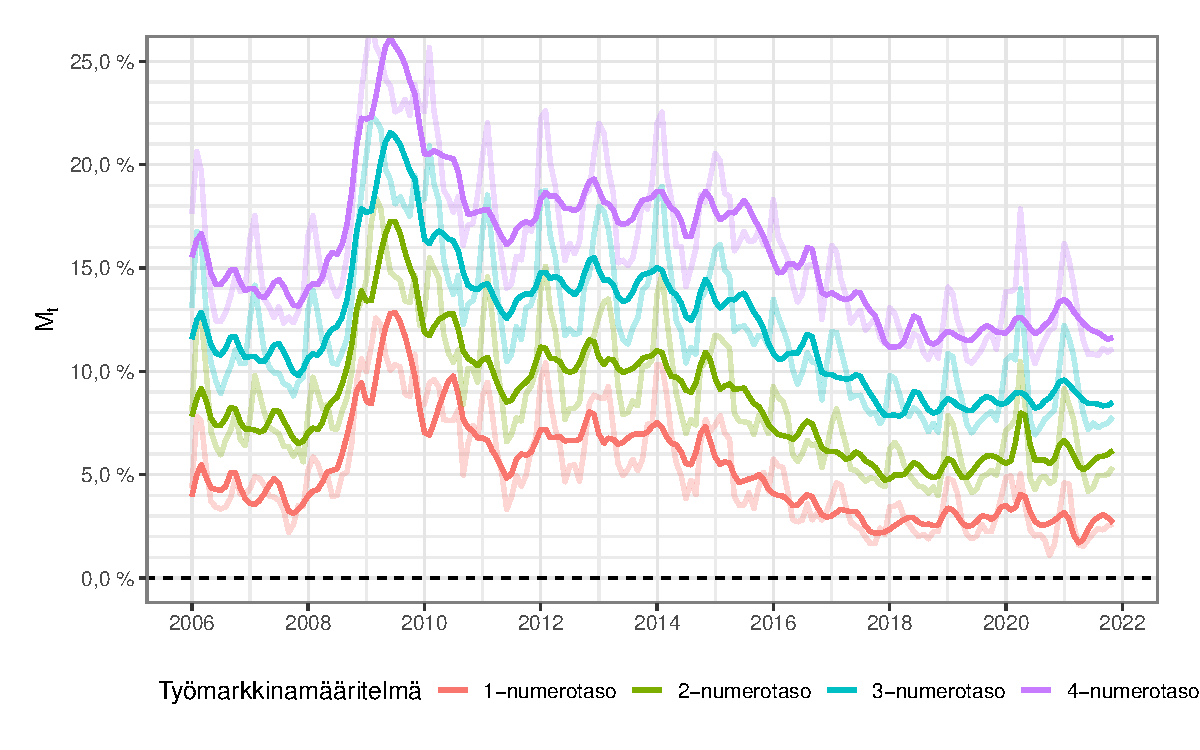
\includegraphics[scale = 0.8]{../kuviot/indeksi_ammateittain.pdf}
    \caption{\textit{Kohtaanto-ongelman suuruutta mittaava indeksi ja sen trendi määrittelemällä työmarkkinat ammateittain. \protect \firstdatamonth - \protect\lastdatamonth. Datalähde: Työnvälitystilasto, Tilastokeskus, taulukko 12ti \protect \cite{svt2011}}}
   \label{fig:kd982}
\end{figure}

Kuvio \ref{fig:kdieksl} esittää alueellisen kohtaannon luoman vajeen työllistymisien määrässä. Mikäli ajattelemme, että kunnat muodostavat omat työmarkkinansa, noin 3 prosentin verran työllistymisistä jää tapahtumatta kuukausittain vuonna 2020 verrattuna tilanteeseen, jossa kuntien väliselle liikkumiselle ei olisi mitään rajoitteita. Vastaava luku seutukunnille on noin 2 prosenttia ja maakunnille noin 1 prosenttia. Kunnittain arvioitu indeksi todennäköisesti yliarvioi kohtaanto-ongelman suuruutta, sillä työttömät työllistyvät myös asuinkuntansa ulkopuolelle \cite{alasalmi2020tyon} ja alueellisen liikkuvuuden rajoite kunnan sisällä on usein pieni. Toisaalta vaikka alueellista liikkuvuutta todellisuudessa luonnollisesti tapahtuu myös maakuntarajojen yli, tämä ei tarkoita, että maakunnittain laskettu indeksi yliarvioisi alueellisen kohtaanto-ongelman suuruutta. Maakunnittain laskettu indeksi nimittäin myös olettaa, ettei maantiede rajoita kohtaantoa maakuntien sisällä. Kurvinen ym. (2019) esimerkiksi arvioivat kyselytutkimuksen perusteella, että pitkäaikaistyöttömien joukossa noin kahdella kolmasosalla työnhakualue on korkeintaan asuinmaakunta ja vajaa viidennes haki työtä ainoastaan asuinkunnastaan.  

Huomiota herättävää on alueellisen kohtaanto-ongelman trendinomainen lasku. Vuonna 2020 työttömien työnhakijoiden jakautuminen alueiden välillä on alueellisen kohtaannon kannalta selkeästi parempi kuin vuonna 2006, ja tänä ajanjaksona alueellisen kohtaannon vuoksi täyttymättä jäävien työpaikkojen osuus on noin puolittunut.

\subsection{Ammatillinen kohtaanto} \label{section:ammatillinen_kohtaanto}

\begin{figure}
\centering
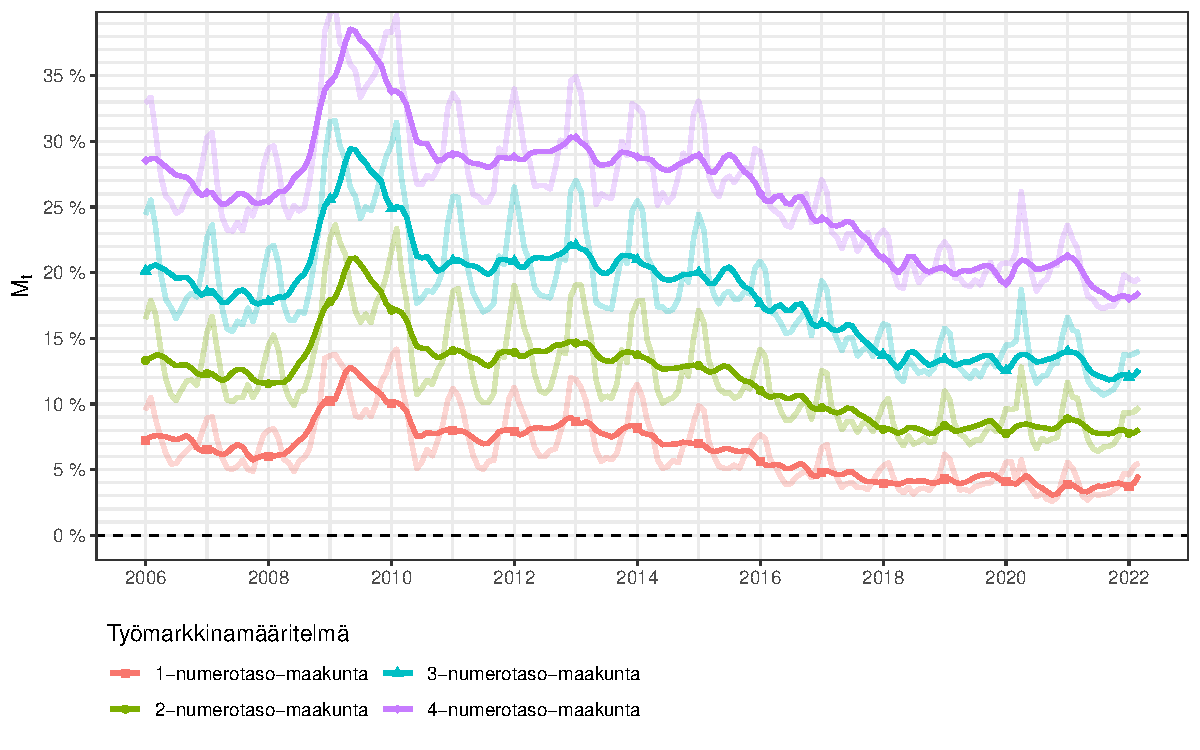
\includegraphics[scale = 0.8]{../kuviot/indeksi_ammateittain_maakunnittain.pdf}
    \caption{\textit{Kohtaanto-ongelman suuruutta mittaava indeksi ja sen trendi määrittelemällä työmarkkinat ammateittain ja maakunnittain. \protect \firstdatamonth - \protect\lastdatamonth. Datalähde: Työnvälitystilasto, Tilastokeskus, taulukko 12ti \protect \cite{svt2011}}}
   \label{fig:l0184hg}
\end{figure}


Tarkastellaan seuraavaksi ammatillista kohtaanto-ongelmaa määrittelemällä työmarkkinat ammattien mukaan. Ammatit ovat luokiteltu Kansallinen Ammattiluokitus 2010 -luokituksen mukaan \cite{tilastokeskus2011ammattiluokitus}. Työnvälitystilaston tiedot tarjoavat luokittelun neljännelle numerotasolle saakka. 1-numerotaso (pääluokkataso) sisältää 10 ammattiluokkaa (luokka X (tuntematon) jätetään pois), 2-numerotaso 43 luokkaa, 3-numerotaso 130 luokkaa ja 4-numerotaso 436 luokkaa. Suurempi numerotaso siis tarkoittaa rajatumpaa työmarkkinan määritelmää ja oletusta rajoitetummasta ammatillisesta liikkuvuudesta. 

Kuvio \ref{fig:kd982} esittää ammatillista kohtaanto-ongelmaa arvioivan indeksin neljälle eri ammattiluokituksen numerotasolle. Jos ajatellaan, että työvoima ei liiku ammattiluokituksen pääluokkien välillä eli esimerkiksi, että entisistä sotilaista ei tule erityisasiantuntijoita, palvelu- ja myyntityöntekijöistä ei tule toimisto- ja asiakaspalvelutyöntekijöitä tai prosessi- ja kuljetustyöntekijöistä ei tule johtajia, niin ammatillisten kohtaanto-ongelmien vuoksi työllistymisien määrä kuukauden aikana väheni vuonna 2019 noin 2–3 prosenttia. Kaksinumeroisella ammattiluokituksella tämä luku on noin 7 prosenttia, kolmenumeroisella noin 10 prosenttia ja nelinumeroisella noin 14 prosenttia.


Kuten alueellisen kohtaannon osalta, ammatillisen kohtaannon luoma vaje työllistymisessä näyttää laskeneen finanssikriisin jälkeen, mutta alueellisesta kohtaannosta poiketen vuonna 2020 työttömien työnhakijoiden ammatit näyttävät vastaavan avoimien työpaikkojen ammatteja yhtä hyvin kuin vuonna 2006. Verrattaessa alueellista ja ammatillista kohtaantoa huomattavaa on myös ammatillisen kohtaanto-ongelmien suurempi herkkyys suhdanteille. Sekä vuonna 2008 alkanut finanssikriisi, että vuonna 2020 alkanut koronaepidemia näkyvät selvemmin ammatillista kohtaanto-ongelmaa arvioivassa indeksissä kuin alueellista kohtaanto-ongelmaa arvioivassa indeksissä. 

\subsection{Alueellinen ja ammatillinen kohtaanto} \label{section:alueellinen ja ammatillinen kohtaanto}

\begin{figure}
\centering
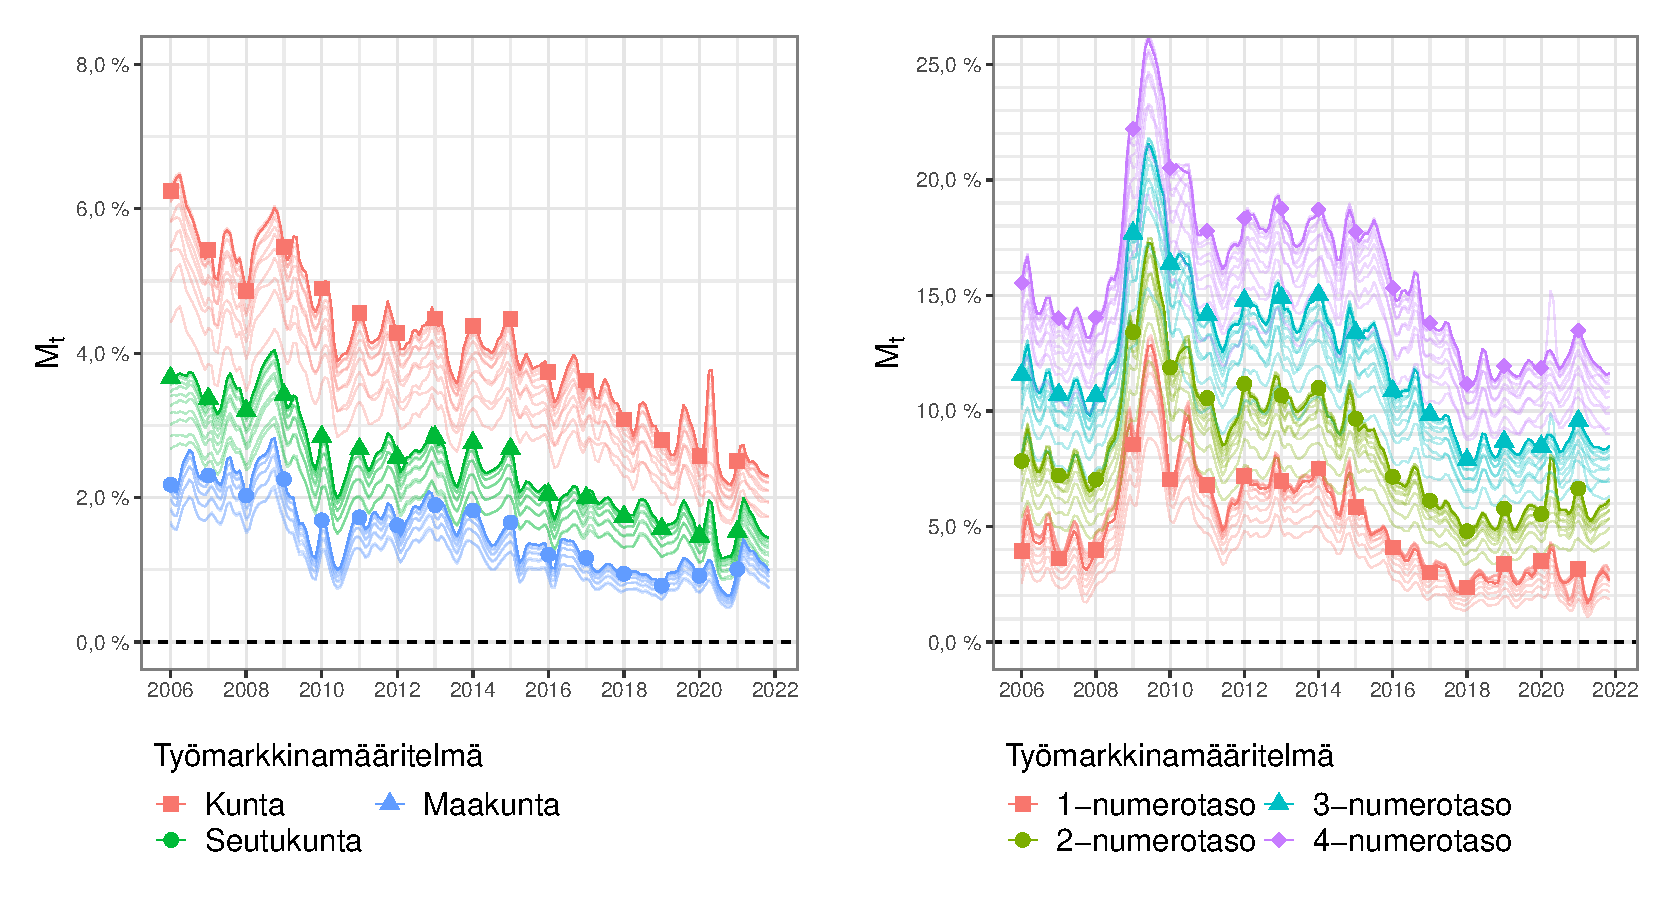
\includegraphics[scale = 0.55]{../kuviot/herkkyys_a.pdf}
    \caption{\textit{Kohtaanto-ongelman suuruutta mittaavan indeksin trendin herkkyys parametrin a arvolle $a \in \{0,25, 0,30, 0,35, 0,40, 0,45, 0,50, 0,55, 0,60, 0,65, 0,70\}$. Indeksi laskettu arvolla $a = 0,5$ tummimmalla värillä. \protect \firstdatamonth - \protect\lastdatamonth. Datalähde: Työnvälitystilasto, Tilastokeskus, taulukko 12ti \protect \cite{svt2011}}}
   \label{fig:ldsdfhg}
\end{figure}

Verrattaessa alueellisten ja ammatillisten kohtaanto-ongelmien suuruutta huomataan, että ammatillinen kohtaanto näyttää vähentävän työllistymisien määrää alueellista kohtaantoa huomattavasti enemmän. Huomaa, että mitä pienemmiksi työmarkkinat määritellään, sitä vähäisempää työmarkkinoiden rajojen ylittävän liikkuvuuden ajatellaan olevan ja sitä suuremmaksi kohtaanto-ongelma arvioidaan. Siten on mielenkiintoista, että esimerkiksi kymmenen ammattiluokkaa eli työmarkkinaa ammatin mukaan määriteltynä näyttävät luovan vastaavansuuruisen kohtaanto-ongelman kuin yli 300 kuntaa eli työmarkkinaa maantieteen mukaan määriteltynä (vertaa Kuvioita \ref{fig:kdieksl} ja \ref{fig:kd982}). Myös \citeA{csahin2014mismatch} käyttäessään yhdysvaltalaista aineistoa aikavälillä 2005–2012 arvioivat, että alueellinen kohtaanto rajoittaa työllistymistä huomattavasti vähemmän kuin ammatillinen kohtaanto. Heidän tuloksiensa mukaan ammattiluokituksen kaksinumerotasolla määritellyt työmarkkinat luovat noin kymmenen kertaa suuremman indeksin arvon kuin piirikuntien mukaan määritellyt työmarkkinat. Hiukan vastaavasti Suomessa ammattiluokituksen kaksinumerotasolla määritellyt työmarkkinat näyttävät luovan noin 6–8 kertaa suuremman kohtaanto-ongelman kuin kuntien mukaan määritellyt työmarkkinat ja noin 2–4 kertaa suuremman kohtaanto-ongelman kuin seutukuntien mukaan määritellyt työmarkkinat. 

\begin{figure}
\centering
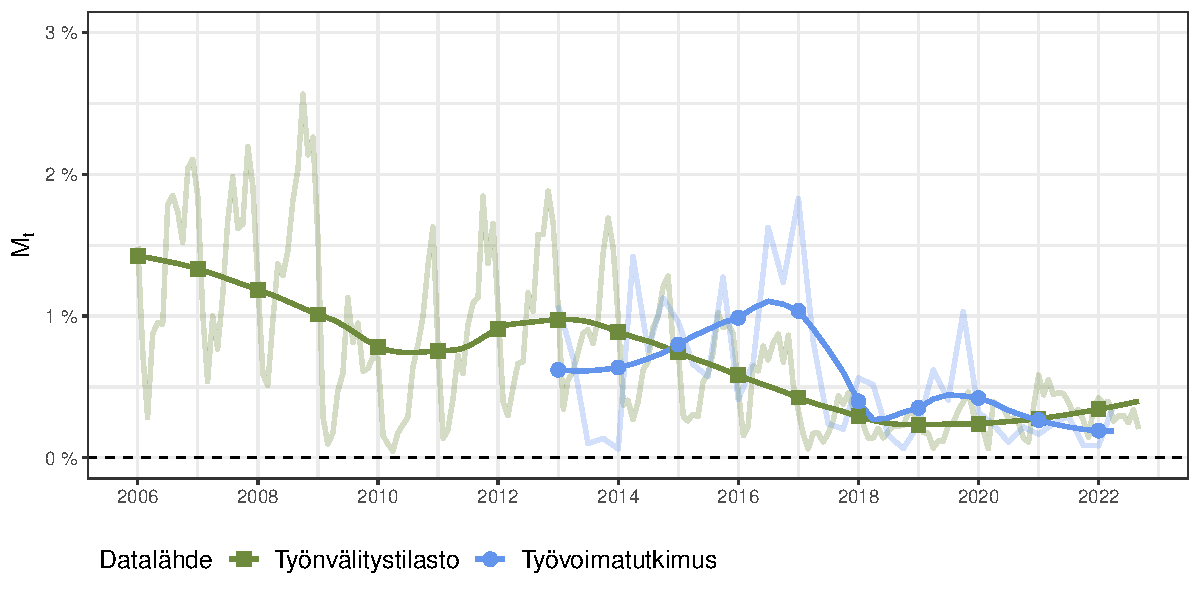
\includegraphics[scale = 0.8]{../kuviot/indeksi_suuralueittain.pdf}
    \caption{\textit{Kohtaanto-ongelman suuruutta mittaava indeksi Työnvälitystilaston ja Työvoimatutkimuksen tiedoilla. Työmarkkina-alueeksi on määritelty suuralue.  Työnvälitystilasto \protect \firstdatamonth - \protect\lastdatamonth. Työvoimatutkimus \protect \firstdataquarter - \protect\lastdataquarter. Datalähde, Työnvälitystilasto, Työvoimatutkimus, Tilastokeskus, taulukot 12ti, 11n1, 11c9  \protect \cite{svt2011}}}
   \label{fig:ld0923g}
\end{figure}

Työmarkkinoita voi määritellä myös sekä alueen että ammatin perusteella. Kuvio \ref{fig:l0184hg} esittää indeksin siten, että työmarkkinat rajautuvat alueellisesti maakuntiin ja ammatillisesti eri ammattiluokkatasoihin. Esimerkiksi ”1-numerotaso-maakunta” käyrä jakaa Suomen siis (10x19=) 190 työmarkkinaan: jokaisessa maakunnassa on kymmenen ammattien pääluokkien muodostamaa työmarkkinaa. Tällaisella työmarkkinoiden määritelmällä työttömien työnhakijoiden liikkumattomuus työmarkkinalta toiselle laski vuonna 2019 kuukausittaisten työllistymisien määrää noin 5 prosentilla. Mielenkiintoista on myös huomata, että määritellessä työmarkkinat sekä ammatillisen että alueellisen ulottuvuuden mukaan, indeksin arvo näyttää ylittävän sen komponenttien summan erityisesti suurilla ammattiluokituksen numerotasoilla tarkasteltuna. Alueelliset ja ammatilliset kohtaanto-ongelmat voivat siis jossain määrin olla komplementaarisia toisilleen. Yleiskuvana alueellisen ja ammatillisen kohtaanto-ongelmien kontribuutio työttömyyteen näyttää kuitenkin laskeneen aikavälillä 2006–2021.

\subsection{Herkkyys} \label{section:herkkyys}

Edeltävissä tarkasteluissa parametrin $a$ arvoksi asetettiin 0,5 aikaisempien tutkimusten ja yksinkertaisuuden vuoksi. Tarkastellaan seuraavaksi, kuinka herkkiä tulokset ovat tälle parametrin arvon valinnalle. Käytetty kohtaantofunktio yleisemmässä muodossa on 
\begin{align}
h_{nt}=v_{nt}^au_{nt}^b,
\end{align}
Suomessa ja maailmalla avoimien työpaikkojen joustoksi ($a$) on arvioitu arvoja välillä 0,2–0,4 ja työttömien määrän joustoksi ($b$) arvoja välillä 0,4–0,7 \cite{lahtonen2006matching, petrongolo2001looking}. Koska Şahinin ym. (2014) kohtaanto-ongelman suuruutta mittaavan indeksin voidaan varmistaa pysyvän arvojen 0 ja 1 välissä (eli käyvän järkeen) vain jos joustot summautuvat yhteen, pitäydyn vakioskaalatuottojen oletuksessa ja asetan $b = 1-a$. Kuvio 4 esittää indeksit useille eri parametrin $a$ arvoille.


Samalla tapaa kuin \citeA{csahin2014mismatch}, huomaamme, että arvon $a = 0,5$ käyttäminen antaa yläraja-arvion kohtaanto-ongelman suuruudesta. Tämän tarkastelun laadullisiin tuloksiin parametrille $a$ annettu arvo ei näytä vaikuttavan. 

Työnvälitystilaston tiedot perustuvat Työ- ja elinkeinotoimistoihin rekisteröityneiden työttömien ja rekisteröityjen avoimien työpaikkojen määriin. Erityisesti siten, mikäli Työ- ja elinkeinotoimistoihin rekisteröityjen avoimien työpaikkojen osuus kaikista työpaikoista vaihtelee alueittain tai ammattiryhmittäin, voi aineiston keruutapa vaikuttaa kohtaanto-ongelmaa mittavaan indeksiin. Tarkastelemmekin tulosten herkkyyttä aineistolähteelle käyttämällä Työvoimatutkimuksen tietoja. Työvoimatutkimus tuottaa tietoa alueellisesti sekä työttömien että avoimien työpaikkojen määrästä kuitenkin vain suuralueittain ja tietoja on saatavilla vain vuodesta 2013 alkaen. Ammatillisen liikkuvuuden tarkastelun osalta sopivaa aineistoa Työvoimatutkimus ei tuota. Kuvio \ref{fig:ld0923g} esittää kohtaanto-ongelman suuruuttaa mittaavan indeksin siten, että työmarkkinan määritelmänä on suuralue (Helsinki-Uusimaa, Etelä-Suomi, Länsi-Suomi, Pohjois- ja Itä-Suomi). Tämän tarkastelun perusteella eri aineistoista lasketut indeksit eivät merkittävästi poikkea toisistaan, mutta Työvoimatutkimuksen tietojen perustella lasketun lyhyen aikasarjan perusteella on vaikea arvioida pidemmän aikavälin trendiä.


\section{Eikö työmarkkinoiden kohtaanto ole heikentynyt?} 

\citeA{pehkonen2018kohtaanto} arvioivat Beveridge-käyriä ja avoimien työpaikkojen täyttymisnopeutta tarkastelemalla työmarkkinoiden kohtaannon heikentyneen 2000-luvulla. Suomen työmarkkinoiden Beveridge-käyrä on myös esitetty kuviossa \ref{fig:ld0923g}. Kohtaannon ammatillista ja alueellista ulottuvuutta mittaava indeksi kuitenkin ehdottaisi, että ammatillinen kohtaanto ei juuri ole heikentynyt, ja että alueellinen kohtaanto olisi parantunut. Myös esimerkiksi \citeA{pyykkonen2016voiko} on arvioinut työttömien työnhakijoiden ja työpaikkojen maantieteellisen keskietäisyyden pienentyneen vuosina 2006–2016. 

\begin{figure}
\centering
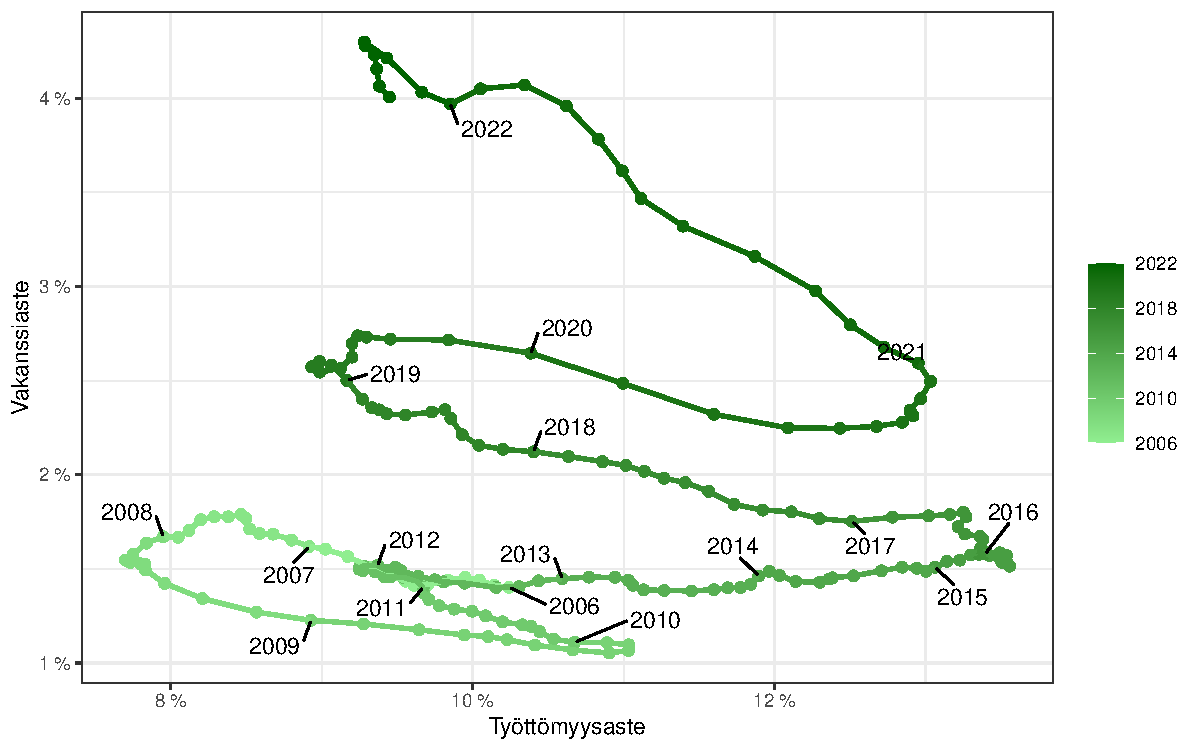
\includegraphics[scale = 0.8]{../kuviot/beveridge_curve.pdf}
    \caption{\textit{Beveridge-käyrä. \protect \firstdatamonth - \protect\lastdatamonth. Työvoimatutkimus \protect \firstdataquarter - \protect\lastdataquarter. Datalähde, Työnvälitystilasto, Tilastokeskus, taulukko 12ti \protect \cite{svt2011}}}
   \label{fig:ld0923g}
\end{figure}

Alueellisen kohtaanto-ongelman pienenemiseen on voinut esimeriksi vaikuttaa kaupungistumisen ja asutuksen keskittymisen jatkuva trendi (esim. \citeA{alasalmi2020tyon}). Kaupungistuminen luonnollisesti keskittää työpaikkoja ja työntekijöitä alueellisesti vähentäen alueellisen liikkuvuuden tarvetta. \citeA{alasalmi2020tyon} myös laskiessaan Beveridge-käyriä erilaisille kuntatyypeille havaitsevat, että kohtaanto-ongelmat ovat suuria ja pahentuneet nimenomaan suurissa kaupungeissa. Yksi keino tutkia avoimien työpaikkojen ja työttömien alueellista keskittymistä on tarkastella, kuinka suuri osa koko maan avoimista työpaikoista tai työttömistä sijaitsee maan suurimmilla työmarkkinoilla. Kuvio \ref{fig:mo034} esittää työvoimaltaan 50 ja 150 suurimaassa kunnassa olevien avoimien työpaikkojen ja työttömien osuuden koko maan avoimista työpaikoista ja työttömistä. Selkeästi yhä suurempi osa avoimista työpaikoista, mutta erityisesti yhä suurempi osa työttömistä sijaitsee työvoimaltaan suurimmissa kunnissa. Tämä avoimien työpaikkojen ja työttömien keskittyminen vähentää alueellisen liikkuvuuden tarvetta ja siten pienentää alueellista kohtaanto-ongelmaa. Tämä näkyy myös alueellista kohtaanto-ongelman suuruutta mittaavassa indeksissä: kun yhä suurempi osa avoimista työpaikoista ja työttömistä keskittyy yhä pienemmälle joukolle alueita, yhä enemmän avoimien työpaikkojen ja työttömien kohtaamisia pystyy tapahtumaan saman työmarkkinan sisällä. Ääritapauksessa, mikäli kaikki avoimet työpaikat ja työttömät keskittyisivät yhdelle alueelle, indeksin arvoksi tulisi nolla.

Ammatillisen kohtaanto-ongelman kehittymisen voisi toisaalta tulkita esimerkiksi finanssikriisin aiheuttamana shokkina työn tarjonnan ja kysynnän ammattijakaumalle, josta toipumiseen ja johon sopeutumiseen työmarkkinoilla on mennyt noin 10 vuotta.

Se, kuinka avoimien työpaikkojen ja työttömien määrät muuttuvat palkkauksiksi ei määräydy kuitenkaan yksin työpaikkojen ja työttömien ammatillisella tai alueellisella sijoittumisella. Käytetty alueellista ja ammatillista kohtaanto-ongelmaa mittaava indeksi olettaa, että työmarkkinoiden sisäinen kohtaannon tehokkuus ei muutu ajanjakson aikana. Tähän työmarkkinoiden sisäisen kohtaannon tehokkuuteen kuitenkin vaikuttaa esimerkiksi työnetsintäkäyttäytyminen, johon puolestaan esimerkiksi työttömien työnhakijoiden ikä ja työllistymisen kannustimet vaikuttavat. Pehkonen ym. (2018) arvioivatkin työllistymisen taloudellisten kannustimien heikentyneen 2000-luvulla. 

\begin{figure}
\centering
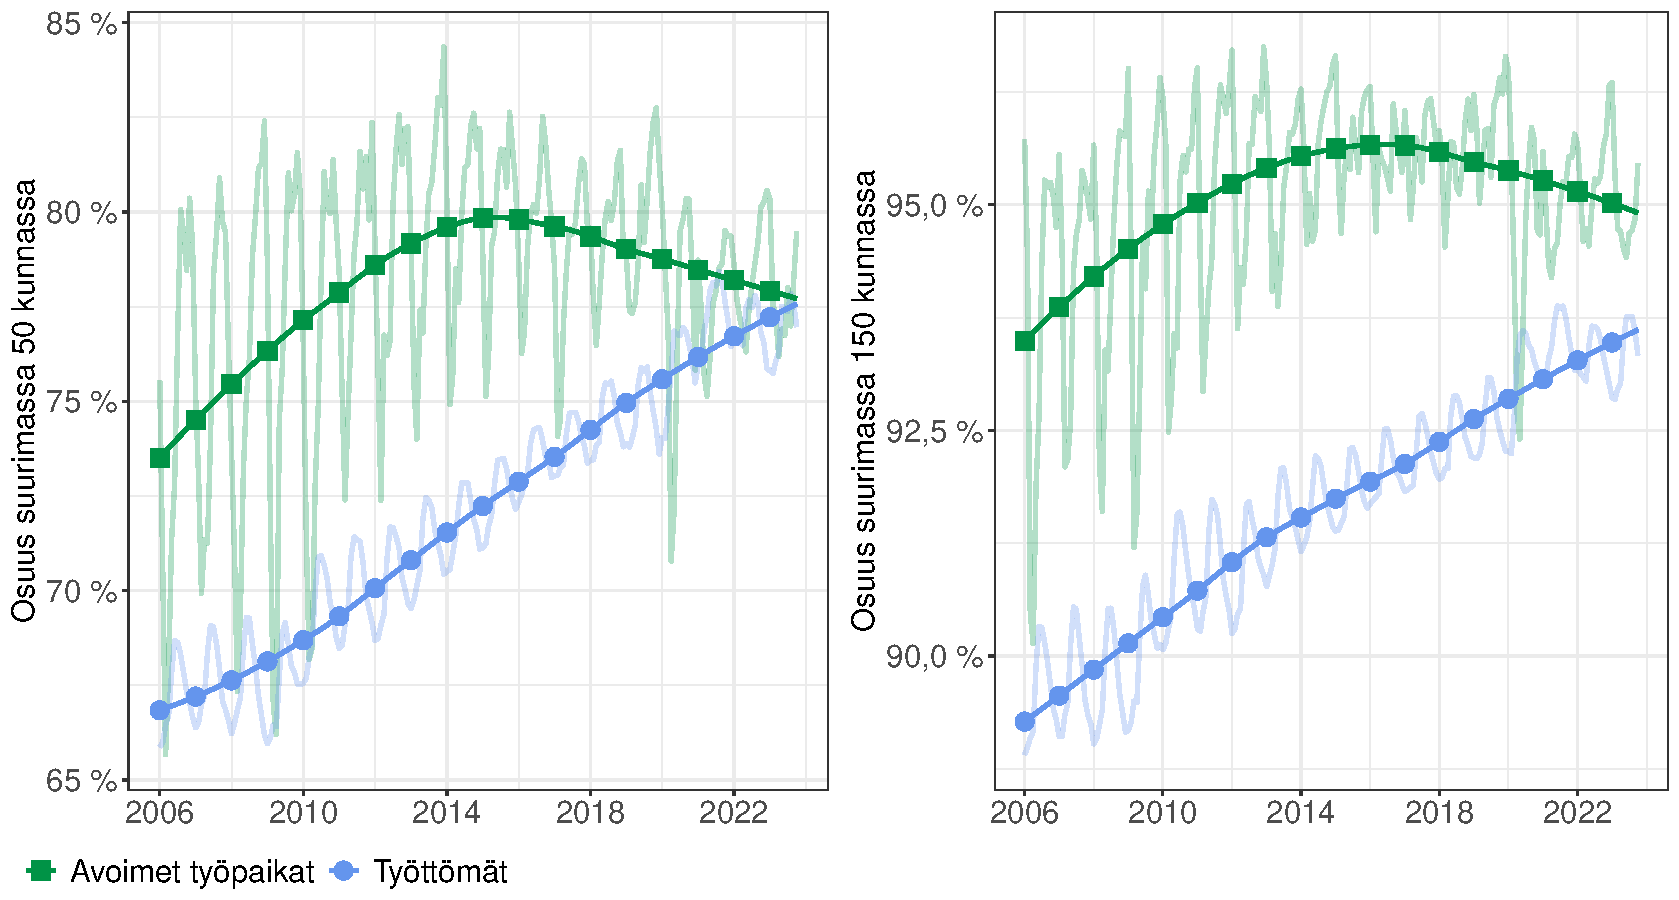
\includegraphics[scale = 0.55]{../kuviot/alueellinen_keskittyminen.pdf}
    \caption{\textit{Osuus koko maan avoimista työpaikoista ja työttömistä 50 ja 150 työvoimaltaan suurimmassa kunnassa. \protect \firstdatamonth - \protect\lastdatamonth. Työvoimatutkimus \protect \firstdataquarter - \protect\lastdataquarter. Datalähde, Työnvälitystilasto, Tilastokeskus, taulukko 12r5 \protect \cite{svt2011}}}
   \label{fig:mo034}
\end{figure}

\section{Lopuksi} 

Tämä teksti arvioi alueellisen ja ammatillisen kohtaanto-ongelmien suuruutta Suomen työmarkkinoilla hyödyntäen Şahinin ym. (2014) kehittämää tekniikkaa. Työmarkkinoiden kohtaanto-ongelmaa arvioitiin ajatusleikillä, jossa koko maan työmarkkinat jaetaan yksittäisiin työmarkkinoihin, joiden välillä ei ole liikkuvuutta. Työttömien työnhakijoiden ja avoimien työpaikkojen epäsuhtaa näillä yksittäisillä työmarkkinoilla verrataan sitten tilanteeseen, jossa työttömän voitaisiin uudelleensijoittaa alueille ja ammatteihin siten, että kohtaanto-ongelma poistuisi. Erilaiset työmarkkinoiden määritelmät alueiden ja ammattiryhmien kokojen suhteen luonnollisesti tuottavat erilaisia tuloksia, mutta esiin nousee myös havaintoja, jotka eivät ole herkkiä tälle määritelmälle. Alueellisen kohtaannon luoma vaje työllistymisen määrässä näyttää trendinomaisesti laskeneen vuodesta 2006 saakka. Myös ammatillinen kohtaanto on parantunut vuoden 2010 jälkeen, mutta lähinnä vuoteen 2020 mennessä saavuttanut tason, jolla se oli vuonna 2006. Tehty tarkastelu vakioi työmarkkinoiden sisäisen kohtaannon tehokkuuden, mikä voi selittää eron työmarkkinoiden kohtaannon usein havaittuun kehitykseen. Yleiskuvana alueellisen ja ammatillisen kohtaannon kontribuutio työttömyyteen näyttää kuitenkin pienentyneen vuoden 2006 jälkeen.

Se, että ammatilliset ja alueelliset kohtaanto-ongelmat eivät näytä huonontuneen vuoteen 2006 verrattuna ei kuitenkaan tarkoita, ettei ammatillisia tai alueellisia kohtaanto-ongelmia olisi. Kohtaanto-ongelman suuruutta mittaava indeksi arvioi alueellisen kohtaamattomuuden vähentävän työllistymisiä kuukauden aikana noin 1–3 prosenttia ja ammatillisen kohtaamattomuuden vähentävän työllistymisiä kuukauden aikana noin 3–12 prosenttia. Työttömien työnhakijoiden epäoptimaalinen ammatillinen sijoittuminen näyttää siis olevan suurempi ongelma kuin työttömien työnhakijoiden epäoptimaalinen alueellinen sijoittuminen. 


 \bibliographystyle{apacite}
\bibliography{kirjasto}

\end{document}